%%%%%%%%%%
% CH5 %
%%%%%%%%%%

\chapter{Les défauts cristallins}
\section{Introduction}
	Le cristal parfait constitue l'état idéal d'un matériau cristallin (énergie interne minimale). Cependa,t dans les cristaux réelles, il y a des imperfections et défauts qui font qu'ils ne sont jamais idéaux. A chaque défaut correspond un excès d'énergie libre par rapport à l'état d'énergie libre minimum. L'ensemble des défauts constitue la \textbf{microstructure}. Certaines propriétés des matériaux sont déterminées par cette microstructure. On distingue trois type de défauts : Les défauts ponctuels (dimension 0), linéaires (dimension 1) et bidimensionnels (dimension 2). 
	
\section{Les défauts ponctuels}
	\begin{wrapfigure}[3]{r}{5cm}
	\vspace{-5mm}
	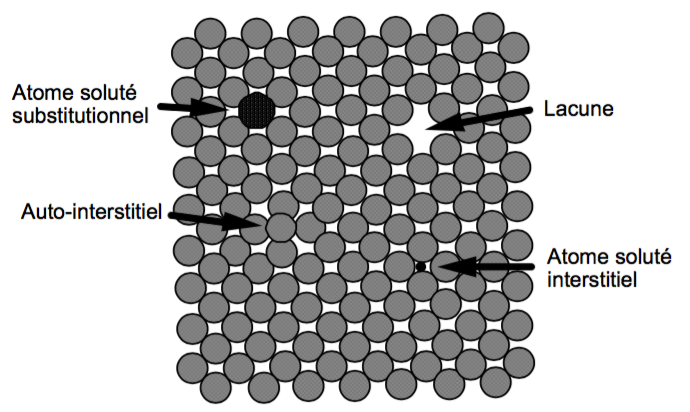
\includegraphics[scale=0.4]{ch5/1}
	\end{wrapfigure}
	Voici la liste des défauts qu'on rencontre dans les cristaux monoatomiques :
	\begin{enumerate}
		\item Les lacunes : absence d'atome sur un site du cristal
		\item Les auto-interstitiels : atome dans une position qui n'est pas un site du cristal
		\item Les interstitiels : atome étranger dans un site qui n'appartient pas au cristal
		\item Les substitutionnels : atome étranger qui remplace un atome du réseau hôte 
	\end{enumerate}
	Dans les cristaux multiatomiques comme les cristaux ioniques, les défauts ponctuels sont plus complexes (on doit maintenir la neutralité électrique). Le déplacement des ions entraîne la formation de paires de défauts voisins : 
	\begin{enumerate}
		\item Paires de \textbf{Schottky} : deux lacunes de nature différente
		\item Paires de \textbf{Frenkel} : une lacune et l'interstitiel correspondant
\end{enumerate}	 
Nous n'approfondissons pas plus. 

	\subsubsection{Les lacunes et les auto-interstitiels}
			Intéressons-nous à la variation de densité avec la température. En première approximation, une lacune augmente l'enthalpie du cristal d'une valeur correspondant au nombre de liaisons devenues insatisfaites. Soit $\Delta H_1$ l'enthalpie de formation d'une lacune et $\Delta S_1$ l'augmentation d'entropie due à la présence de lacune. On a alors la relation 
			\begin{equation}
				\Delta G_1 = \Delta H_1 - T\Delta S_1
			\end{equation}
			Si $N_t$ est le nombre de sites du cristal et $N_1$ le nombre de lacunes, la concentration en lacunes vaut $C_1 = \frac{N_1}{N_t}$ et s'exprime comme
			\begin{equation}
				C_1 = \exp \left( -\frac{\Delta G_1}{k_B T} \right) = \exp \left( \frac{\Delta S_1}{k_B} \right)\exp \left( -\frac{\Delta H_1}{k_B T} \right)
			\end{equation}
			La relation montre qu'il y a toujours une certaine concentration de lacunes qui augmente avec la température. Pour illustrer, dans une maille CFC l'énergie de formation vaut $1\, eV$. On calcule alors que la concentration à $300\, K$ vaut environ $10^{-22}$ alors qu'à $1300\, K$ elle passe à $10^{-5}$, c'est impressionnant ! En pratique, la présence de lacune permet aux atomes voisins de sauter et d'ainsi déplacer la lacune sur le réseau. C'est comme ça qu'est gouverné la mobilité des atomes dans le réseau. \\
			Le principe est le même pour les auto-inerstitiels sauf que leur enthalpie de formation est 4 fois plus grande (dans une CFC) que celle des lacunes, menant à une concentration négligeable à toute température. Le changement de concentration avec la température est permis par l'émission de lacunes par des \textbf{sources} ou leur absorption par des \textbf{puits}. 
			
	\subsection{Les sites interstitiels dans les structures cubiques}
		\begin{wrapfigure}[6]{l}{7cm}
	\vspace{-5mm}
	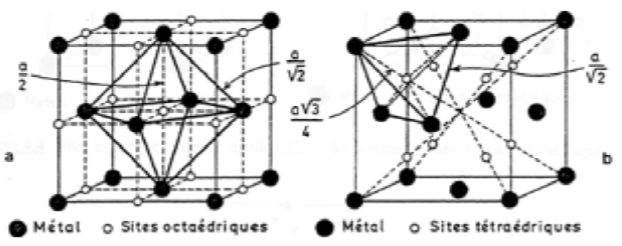
\includegraphics[scale=0.6]{ch5/2}
	\end{wrapfigure}
	On se rappelle du chapitre sur les structures CFC, CC et HC, qui sont celles de la plupart des métaux purs. Elles sont formés par l'empilement de sphères dures en contact les unes avec les autres. Comment les atomes de petite taille tape l'incruste ? On représente les CFC et CC comme un cube avec un atome à chaque sommet + un atome au milieu de chaque face pour le CFC et un atome au centre du cube pour le CC. \\
	Notons $R_A$ le rayon des sphères dures et étudions la forme géométrique représenté ci-contre (CFC). On trouve pour le \textbf{CFC} deux types de sites : 
	\begin{enumerate}
		\item des sites \textbf{octaédriques}, délimités par 6 atomes occupant les sommets d'un octaèdre
		\item des sites \textbf{tétraédriques}, définis par 4 atomes au sommet d'un tétraèdre
	\end{enumerate}
	Les deux types de polyèdres sont réguliers. Les sites octaédriques occupent le centre du cube et les milieux des arrêtes. Il y a un total de 4 sites octaédriques par maille (1 au centre + 12/4 aux arrêtes). Le rayon $R_0$ laissé à l'atome étranger vaut $0.414\, R_A$. Il y a 8 sites tétraédriques par maille (un huitième du cube = site). Le rayon libre dans ce cas est de $R_T = 0.225\, R_A$. On voit donc que l'octaédrique laisse un plus grand espace aux étrangers. \\
	\begin{wrapfigure}[6]{r}{7cm}
	\vspace{-10mm}
	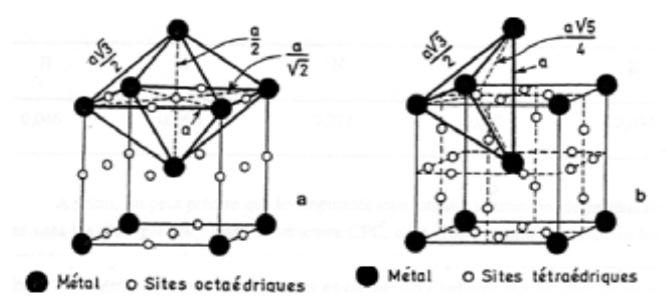
\includegraphics[scale=0.6]{ch5/3}
	\end{wrapfigure}
	Dans le cas de la structure \textbf{CC}, les polyèdres ne sont PLUS réguliers. Les sites octaédriques occupent les centres des faces, ainsi que le milieu des arrêtes. La distance du centre aux quatre coins du carré est plus grande que la distance entre les sommets de la pyramide. On a ainsi un rayon disponible de seulement $0.155\, R_A$ entre les sommets de la pyramide alors que dans la direction des 4 cotés du triangle on est à $0.633\, R_A$. Les sites tétraédriques se trouvent sur les faces du cube à mi-distance entre deux sites octaédriques. Il n'est pas régulier mais on peut y inscrire une sphère de rayon $0.211\, R_A$.
	
	\subsubsection{Solubilité}
		Pour qu'un atome étranger ne déforme pas le réseau, il faut que son rayon soit inférieur à $R_0$ ou $R_T$. Les seuls atomes de tailles suffisamment petites capable d'entrer en solution d'insertion sont $H,N,O,C$ et $B$. En fait, seul l'hydrogène est assez petit, les autres provoquent une distorsion du réseau. Les impuretés se placeront dans les interstices les plus grands. Dans la maille CFC cela correspond aux sites octaédriques alors que dans la CC c'est plus complexe dû à l'asymétrie des sites. Cependant, on observe qu'ils se placent préférentiellement dans les octaédrique, sûrement dû au seul contact avec deux atomes (distances entre 4 côtés du carré grands) alors que le tétraédrique en induit 4. \\
	On peut prévoir que la solubilité sera d'autant plus grande que la distorsion du cristal est faible. En effet, l'énergie de distorsion est une contribution positive à l'enthalpie libre du cristal. Si cette énergie devient trop grande, les nouvelles impuretés auront tendance à former un solide distinct de l'original. On en conclu que la solubilité des interstitiels est plus grande dans une CFC que dans une CC, alors que le volume totale des interstices est plus grand dans le CC mais leur nombre plus grand fait qu'ils sont plus petit. \\
		
		\begin{wrapfigure}[9]{r}{7cm}
	\vspace{-10mm}
	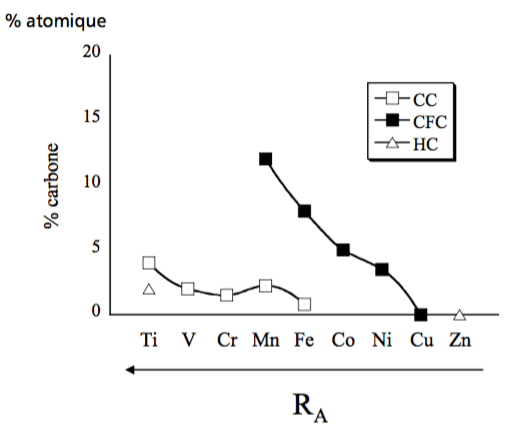
\includegraphics[scale=0.6]{ch5/4}
	\end{wrapfigure}
		Le cas du fer est particulièrement intéressant car il présente une structure CFC (austénite) à haute température et une structure CC (ferrite) à basse température. Les aciers sont issus de la combinaison de fer et de carbone (max 2\% en poids). La solubilité du carbone dans la structure CFC sera plus grande que dans la structure CC. Lors du réchauffement, tout le carbone présent dans les aciers peut entrer facilement en solution avec l'austénite. Mais lors du refroidissement, le carbone sera en excès, donnant lieu à un précipité cristallin différent qui est dans les cas les plus simple un carbure de fer $Fe_3C$ (cémentite). Ces précipités affectent les propriétés mécaniques de l'acier et leur taille et forme dépendent sensiblement des conditions de refroidissement de l'acier. \\
		Dernièrement, il n'y a pas que le rayon atomique qui compte. En effet, une affinité chimique élevé entre l'élément interstitiel et l'élément métallique favorise la précipitation de composés distincts, limitant ainsi la teneur de l'élément en solution solide. C'est ainsi qu'on ne retrouve pratiquement pas d'$O_2$ dans le fer en raison de l'oxydation, alors que le rayon est inférieur à celui du carbone. 

\section{Les défauts linéaires : les dislocations}
	\subsection{Le concept de dislocation}
	Ce sont, pour l'essentiel, les propriétés des dislocations qui gouvernent les phénomènes de déformation plastique des matériaux cristallins. La dislocation apparaît dans un matériau lorsqu'une partie du matériau se déplace par rapport à l'autre par \textbf{glissement} le long d'un plan cristallin. Elle désigne le défaut linéaire à la frontière entre les deux parties. 
	
	\newpage
	\subsubsection{Dislocation coin}
	\begin{wrapfigure}[12]{l}{4cm}
	\vspace{-5mm}
	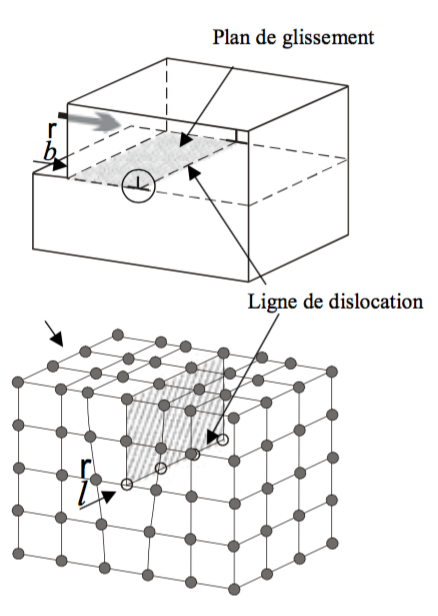
\includegraphics[scale=0.5]{ch5/5}
	\end{wrapfigure}
	Une partie du cristal est supposé s'être déplacée par rapport à l'autre sur une \textit{distance égale à la distance séparant deux noeuds équivalents du réseau}. Le glissement se fait suivant une direction parallèle à une direction du réseau, le long d'un plan particulier. Le \textbf{vecteur de Burger} $\mathbf{\vec{b}}$ représente cette direction. Aucun défaut n'est crée le long du plan de glissement. Cependant, une ligne de défaut se crée à la frontière entre la partie du plan qui se déplace et l'autre. On l'appelle \textbf{dislocation coin} ("edge dislocation"). Le défaut peut être représenté comme étant situé au voisinage de l'arête d'un demi-plan supplémentaire inséré entre deux plans du réseau. La partie la plus déformée sera alors appelé \textbf{coeur de la dislocation}. L'orientation de la ligne de dislocation peut être décrite par un vecteur unitaire $\mathbf{vec{l}}$. Dans le cas d'une dislocation coin, $\vec{l}$ et $\vec{b}$ sont perpendiculaires. 
	
	\subsubsection{Dislocation vis}
	\begin{wrapfigure}[7]{r}{7.5cm}
	\vspace{-5mm}
	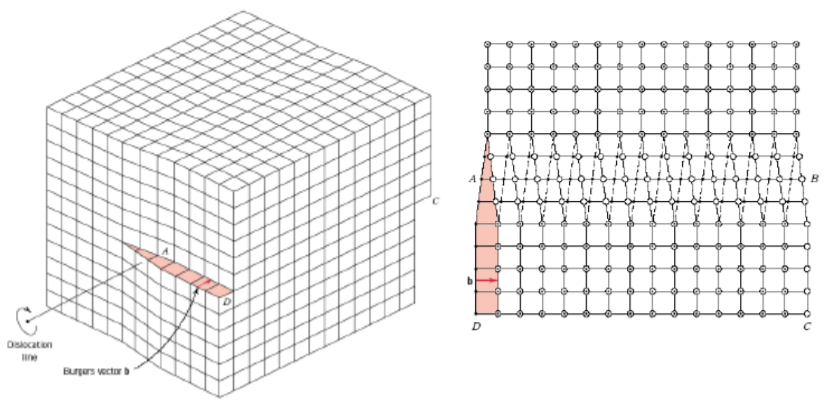
\includegraphics[scale=0.5]{ch5/6}
	\end{wrapfigure}
	La dislocation vis ("screw dislocation") est le résultat d'un glissement d'une partie du cristal le long d'un plan, à la différence que cette fois la ligne de déformation est parallèle au vecteur de Burger. On peut voir le vecteur $\vec{l}$ comme une vis qui tourne comme sur le schéma. Les atomes les plus au centre sont disposé de telle manière à former une hélice ou une vis. 
	
	\subsubsection{Dislocation mixte}
	\begin{wrapfigure}[6]{l}{6.5cm}
	\vspace{-5mm}
	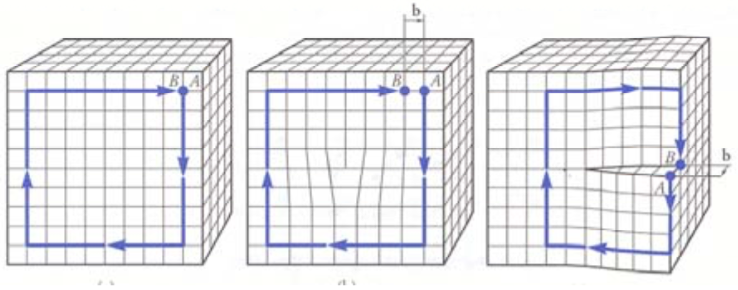
\includegraphics[scale=0.5]{ch5/7}
	\end{wrapfigure}
	C'est le cas le plus général qui est la combinaison des deux dislocations précédentes. Dans ce cas, le vecteur $\vec{l}$ change d'orientation continuellement alors que le vecteur $\vec{b}$ à une orientation fixe. Certaine partie de la dislocation sont donc vis et d'autres coin. 
	Le vecteur de Burger est le défaut de fermeture d'un circuit que l'on tracerait autour de la dislocation, dans un plan perpendiculaire. 
	
	\subsubsection{Energie de dislocation}
		La présence d'une dislocation entraîne un excès d'énergie libre puisqu'elles perturbent les positions d'équilibre des atomes. On montre que cette énergie est directement proportionnelle à $b^2$. Pour avoir le $b$ le plus petit, on applique les déformations suivant une direction compacte du réseau, incluse dans un plan compacte. De ce fait, le vecteur de Burger sera parallèle aux directions $<1\, 1\, 0>$ dans les CFC et $<1\, 1\, 1>$ dans les CC. 
		
	\subsubsection{Densité de dislocations}
		On a un déséquilibre énergétique dû à la présence de dislocations dans le réseau, en élevant la température, on facilite le retour à l'énergie libre minimale. Dans les métaux, cet excès est relativement faible, il est donc impossible d'éliminer toutes les dislocations même après un long maintien à haute température. La densité de dislocation se situe alors typiquement entre $10^{-6}$ et $10^{-7}$. Les croisements entre dislocations forment des \textbf{points d'ancrage} qui entrave le déplacement de celles-ci.
	
	\subsection{Mouvement des dislocations}
		\subsubsection{Le glissement}
			Le déplacement d'une ligne de dislocation d'une distance égale à une fois le vecteur de Burger ne provoque que de faibles déplacements des atomes au voisinage du coeur de dislocation. On dit de ce mouvement \textbf{glissement de dislocation}. Le plan le long duquel s'effectue le glissement est le plan de glissement, qui dans le cas d'une dislocation coin est formé par $\vec{b}$ et $\vec{l}$. On a une déformation permanente lorsque la déformation se déplace sur l'étendu totale d'un plan traversant le cristal. C'est moins intuitif pour la dislocation vis.  \\
	\begin{wrapfigure}[10]{l}{4.5cm}
	\vspace{-9mm}
	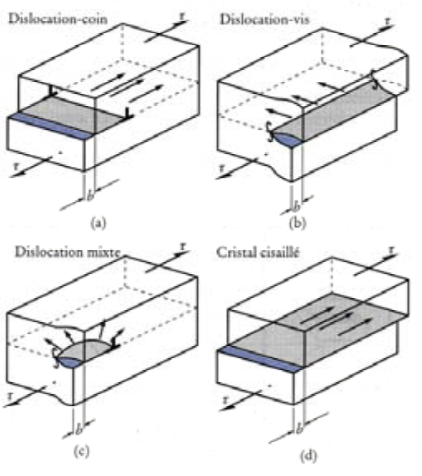
\includegraphics[scale=0.6]{ch5/8}
	\end{wrapfigure}
	Le déplacement est un phénomène aisé (ils sont petits). Le travail total dépensé à faire glisser la dislocation est plus faible que le travail mis en oeuvre pour déplacer toute une partie du cristal pour une distance de 1x $\vec{b}$. On peut voir ça comme quand on pousse un tapis avec le pied, déplacer la bosse fatigue moins que tirer tout le tapis. La composante de la force appliquée qui fait bouger une dislocation est la \textbf{composante de cisaillement dans le plan de glissement}. \\
	On peut voir ci-contre, qu'une même déformation macroscopique peut être atteinte par des mouvements de dislocations différentes, par un même $\vec{b}$. La dislocation se déplace toujours perpendiculairement à sa ligne. 
	
	\subsubsection{Le glissement dévié}
		\begin{wrapfigure}[6]{l}{3.5cm}
		\vspace{-5mm}
		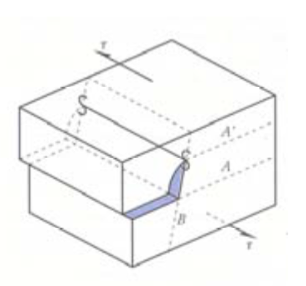
\includegraphics[scale=0.65]{ch5/9}
		\end{wrapfigure}
		Une dislocation vis peut glisser selon n'importe quel plan contenant la ligne de déplacement. En conséquence, elle peut changer de plan de glissement durant son déplacement, elle passera d'un plan compact à un autre. C'est ce changement de plan qu'on appelle \textbf{glissement dévié} et influence fortement la faculté de déformation plastique des matériaux cristallin. 
		
	\subsubsection{La montée}
		\begin{wrapfigure}[6]{l}{4.5cm}
		\vspace{-5mm}
		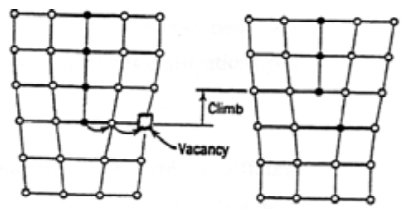
\includegraphics[scale=0.6]{ch5/10}
		\end{wrapfigure}
		Appliquons une contrainte de traction ou de compression suivant le vecteur de Burgers d'une dislocation coin. Le cristal pourra se déformer à condition que le demi-plan supplémentaire puisse se déplacer parallèlement à lui-même par un mouvement vers le haut ou vers le bas. Vers le bas si une lacune présente dans le réseau vient substituer un atome occupant un site sur l'arrête du demi-plan et vers le bas si on procède à une addition d'un atome supplémentaire sur l'arrête du demi-plan (formation d'une lacune sur le réseau). Les deux mouvements sont appelés \textbf{montée d'une dislocation} et ne concerne que les dislocations coins. Le mouvement est d'autant plus facile que la concentration en lacune est élevé, donc à haute température.  
			
	\subsection{Multiplication des dislocations}
		Si toutes les dislocations se déplaçait jusqu'à sortir du cristal, la déformation provoquée sera plus faible que celle introduite par déformation plastique. D'ailleurs dans cette dernière déformation, la densité de dislocations augmente considérablement. Il y a donc un mécanisme de multiplication des dislocations. 
		
		\subsubsection{Le moulin de Frank et Read}
			\begin{wrapfigure}[8]{l}{6cm}
		\vspace{-5mm}
		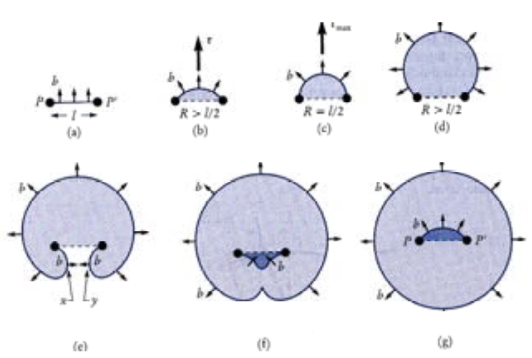
\includegraphics[scale=0.6]{ch5/11}
		\end{wrapfigure}
			Le déplacement des dislocations peut être contrecarré par des obstacles (précipités, noeuds ...). Soit un segment de dislocation de longueur $l$, encré en deux points P et P'. On applique une contrainte pour la déformer et on montre que la force est inversément proportionnelle au rayon de courbure. Donc, jusqu'à un rayon de 1/2 la force augmente (rayon de courbure diminue) puis reste constante pour que le rayon de courbure augmente spontanément. Les segments x et y finissent par se toucher et s'annulent puisque les vecteurs de Burger sont opposés. On a alors une boucle fermé qui se déplace alors que le segment initial va recommencer le processus. C'est le mécanisme de Frank et Read. 
			
\section{Les défauts bidimensionnels : joints de grains, macles et défauts d'empilement}
	\subsubsection{Les joints de grains}
		\begin{wrapfigure}[6]{r}{3cm}
		\vspace{-5mm}
		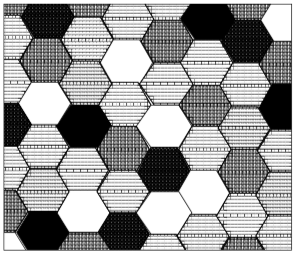
\includegraphics[scale=0.6]{ch5/12}
		\end{wrapfigure}
		Les matériaux usuels sont constitué de nombreux cristaux d'orientation cristallographique différente que l'on nomme \textbf{grains}. Les joints de grains sont des défauts résultant de la rencontre de deux grains cristallins d'orientation différente. La nature du joint de grains dépend de l'écart d'orientation entre les grains en contact. 
		
		\subsubsection{Les fautes d'empilements et macles}
			\begin{wrapfigure}[8]{l}{3.5cm}
		\vspace{-5mm}
		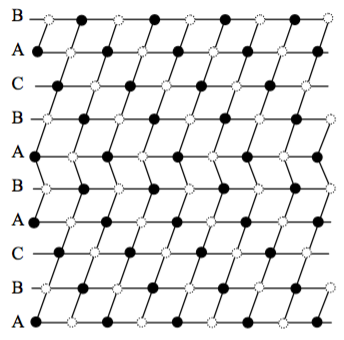
\includegraphics[scale=0.6]{ch5/13}
		\end{wrapfigure}
		On se limite au cas d'une structure CFC où on se rappelle que l'empilement se faisait suivant le plan compact ${1\, 1\, 1}$ et suivant l'ordre ABCABC. La faute d'empilement correspond en un non respect de cette règle d'empilement. Remarquons que l'introduction d'une erreur d'empilement tous les deux plans compact donne la structure HC. \\
		Un macle est un joint de grain très particulier. L'ordre d'empilement de part et d'autre du plan de macle sont des "images miroirs". Un joint de macle est suivi d'un 2e qui ramène le cristal dans l'orientation de la séquence de départ (v. images ci-dessous).\\
		
		\begin{minipage}{0.45\textwidth}
		\begin{flushright}
		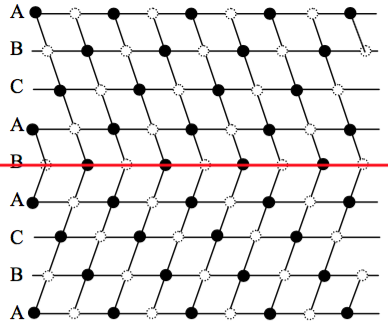
\includegraphics[scale=0.5]{ch5/14}
		\end{flushright}
		\end{minipage}
		\begin{minipage}{0.5\textwidth}
		\begin{flushleft}
		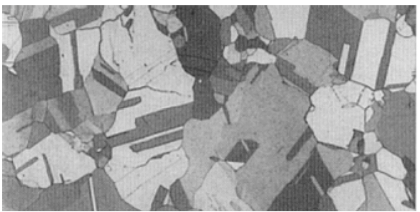
\includegraphics[scale=0.8]{ch5/15}
		\end{flushleft}
		\end{minipage}